\chapter{Design}
\epigraph{``Another quote.''}{\vspace{10pt}Another Author}
\label{chapter:design}
\newpage

This chapter presents the models use to test the hipotesis. As the ground truth a CNN estimator is selected to explore the the capability of a model to learn and estimate from the acoustic signals the location of an object in a tridimentional space. The input trasformation to images and the changes requiered to the red to work as an estimator are mentioned. Also, in this section the design of a memory eficient network in the form of an ESN estimator is presented. A justification for The ESN model architecture selection, the input trasformation and training and evaluation process is provided. Finally the Beamforming mechanism intended to compress information and highlight acoustic echoes from specific regions is described in detail.

\section{CNN Estimator}

The related work presented in seccion 2.6.2 provide insights respect the potential use of neural network to estimate the location of an object using acoustic echoes, and considering the especific findings in \cite{echosense} is that a metric is extrapolated for the magnitude of estimation error. Due the fact that the dataset was new and unexplored, the model choose to establish a reference point was a CNN, this with the premise that a CNN have enogh representational capacity to learn from an especific acostic trasformation the function that maps the input features to espatial coordinates, providing valuable information if our original goals can be achieved with a more restricted network as is the case of an ESN. 

\subsection{Log-Mel spectrogram as images}

To employ a CNN to train on the dataset a Log-Mel transformation is perform to the audio signals in order to obtain spectograms of images that can be use as input for the network. The audio signals have length of 35000 samples, and a Short-Time Fourier Transform (STFT) using a window length of 2048 that provide a good frequency representation and a window step of 512 samples the frequency frames are obtained as detailed in equation \ref{eq:fframes} resulting in 68 frames. An aditional aditional mel filterbank is used to compress espectral data into 128 bands to help machine learning models to process the information more eficienty \cite{log_mel_convolutional}

\begin{equation}
\label{eq:fframes}
\text{Frequency frames} = \frac{signal\_length}{window\_step} 
\end{equation}

Finally to reduce feature variance in the mel bands a logaritmic trasformation is perform. The resulting log-mel matrix is transform to images of 570x370 pixes per location-orientation as the one show in Figure \ref{spectogram4ch}. 

\begin{figure}[!htb]
        \begin{center}        
            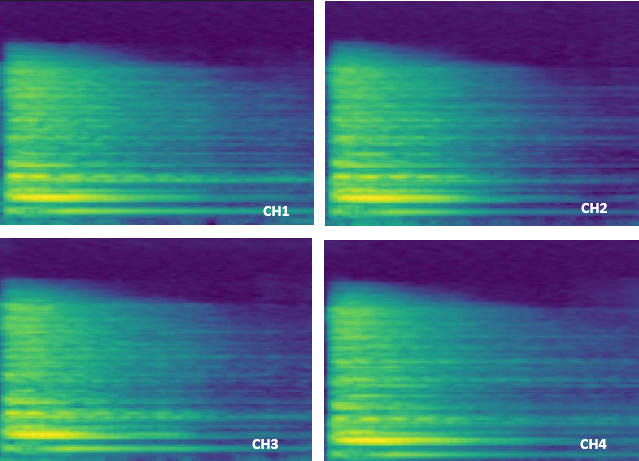
\includegraphics[height=10cm, width=15cm]{../img/4channelSpec.png}
            \caption{Log-Mel spectograms correspondig of the four channels of signals captured at session 1, location X=22.8, Y=-0.94 , Z=-9.43 and orientation 50 degrees.}
        \label{spectogram4ch}                         
        \end{center}
\end{figure}



\subsection{CNN Architecture}

The model architecture selected for the task of classifying and estimating the location–orientation of the cube inside the measure box was the ResNet‑18 network, chosen for its robustness, simplicity, and suitability for inference in resource‑constrained environments \cite{Resnetwhy} (like the present in google colab notebooks). Two modifications were applied to the standard network structure. First, the input layer was extended to accept a stack of four RGB images, one corresponding to each audio channel. Second, for the regression task, the softmax output layer was replaced with a single output feature using a sigmoid activation function.

\subsection{CNN Training and Evaluation}

The network is trained to reduce the Mean Square Error for regression tasks, the optimization algorithm is the Adaptive Momentum Estimation. 
The training loop runs for 40 epochs, following the five fold paradigm, the training portion contains four folds and the test set is the remaining fold for a partitioning of 80:20 percent ratio. The epoch process happens in batches of size 32, for a total of 350 batches per epoch.
The target values for X, Y and Z are normalized before the training process. A min-max normalization scales the value into the range $[0,1]$ to fit the output response of the network. For X and Y an extra normalization step is performed since the path between these points describes a circular trajectory, the robotic arm’s rotational movement at constant angular increments of 10 degrees causes the projections of these coordinates to be expressed as multiples of sine and cosine functions. Consequently, the distribution along the coordinate axes is not uniform and requires an arcsin transformation shown in equation \ref{eq:normalization} in order to result in a equidistant mapping.


\begin{equation}
\label{eq:normalization}
label\_arcnorm =  \frac{\arcsin(2label\_norm - 1) + \frac{\pi}{2}}{\pi}
\end{equation}

After training the model is change to evaluation mode and the test set procesed to obtain the output from the estimator. A denormalization in the inverse funtion of equation \ref{eq:normalization} is perform and the results is use to calculate the estimation error as the diference with the ground truth coordinate value. The MAE, the error distribution and the percentage estimations per error range are calculated with the test results. 


\section{ESN Estimator}

The ESN model is particularly efective learning from sequential data capable of learning from complex sequences of values due it rich temporal memory non linear dynamics, both atributes that share with the RNN but without the drawbacks of training the recurrent part of the network. The ESN tend to be a compact network, that the reason it is proposed in this document as a memory efficient model well suited to work as an estimator. 

\subsection{Mel spectrogram as sequence}

For the ESN, the audio channels are cropped to only 20 000 sample to reduce the long tail with low signal power, the resulting signals are trasformend into sequence of Mel values, for this task, in similar way as te process described in seccion 5.1.1 a Short-Time Fourier Transform (STFT) using a window length of 1024 frames this time for speed up the transformation process and a window step of 512 samples was employ to obtain 40 frames. The Mel bank filter compress the data into 128 bands, a resulution adecuate for acoustic scene identification and direction of arrival identification \cite{numelbands}. The resulting bands are proceced by a decibel trasformation. The resulting spectrum sequence have a length of 40 values with 128 features per channel. A final step of feature scaling using min-max normalization is performed on the input features as a good practice to avoid problems with high magnitude variation between input values.

\subsection{ESN Architecture}

The development of the ESN architecture begins with the vanilla flavor of the ESN all set to work as an clasifier. for exploration and evaluation the network is first configure as an clasifier due that this task is easier than regression \cite{vapnikstatistical}, so the earlier evaluations and changes on the ESN are conducted in it clasification mode. 

The base ESN had as input four mel spectograms sequences of 128 bands each, for a total of 512 inputs, the neurons use tanh activation function for reservoir and the feedforward network. The output softmax layer clasifiy into 26 classes based on the session in which the audio is recorded.

The parameters for the networks are show in the table \ref{tab:esn_parameters}:

\begin{table}[htbp]
\centering
\caption{Key parameters of an Echo State Network (ESN)}
\label{tab:esn_parameters}
\begin{tabular}{lp{10cm}}
\hline
\textbf{Parameter} & \textbf{Description} \\
\hline
\texttt{reservoir size} & The total number of internal recurrent neurons within the reservoir, determining the dimensional capacity to represent complex dynamical states. \\
\texttt{spectral radius} & The largest absolute eigenvalue of the recurrent weight matrix, governing stability, memory decay rate, and the Echo State Property (ESP). \\
\texttt{sparsity} & The fraction of zero-weight connections within the reservoir matrix, decoupling internal sub-dynamics and lowering computation costs per update. \\
\texttt{leaky rate} & The leaking integration parameter $[0, 1]$, controlling how fast the reseirvoir forget previous states. \\
\hline
\end{tabular}
\end{table}

The spectral radius that control how memory decay in the reservoir is desire to have it as hier as posible in order that the network present a long term memory behaviour, the maximun value recommended had a boundary of 1 to ensure the ESP to warranty that the internal states of the reservoir will converge over time avoiding instability. For the ESN presented in this work a value of 0.99 was choose as spectral radius for the reservoir matrix. The leaky rate also controlls how fast the reservoir forget and it set to 0.1 to avoid memory loss and keep as much as posible of the history of the input sequence in the reservoir.

The sparity is keep to 0.1 for mantain a high conectivity of neurons in the reservoir. For the reservoir size, as the value set to this parameter is expensive in memory during training and is a direct factor determining the amount of trainable weights in the feedforward network, a search is perform to find a value with a good ration of acurracy/size. The figure \ref{reservoirsize} show the curve of the results obtained for the acuracy vs the reservoir size and can be observe that the acuracy increase as the reservoir size increase until reach the 1500 neurons, after this point increasing the size of the reservoir do not necesarily correspond to an improvement in the performance of the network.

\begin{figure}[!htb]
        \begin{center}        
            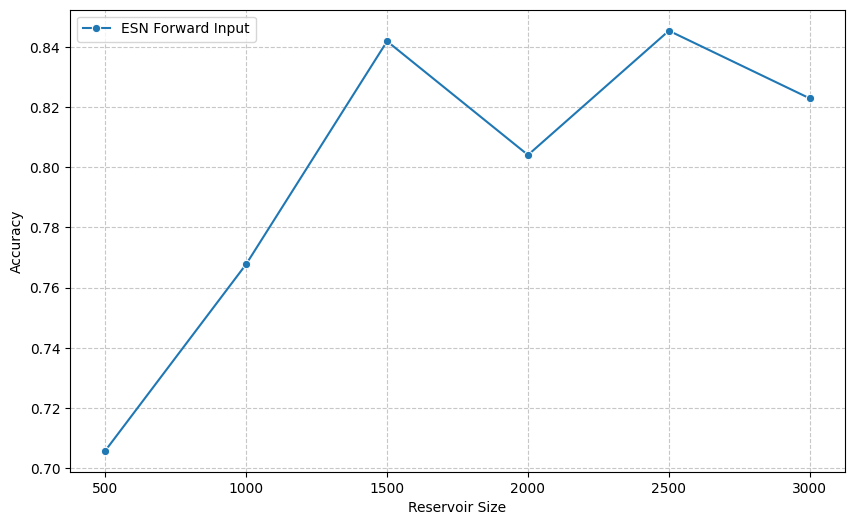
\includegraphics[height=8cm, width=13cm]{../img/reservoirsize.png}
            \caption{Network accuracy vs. reservoir size for 50 epochs runs.}
        \label{reservoirsize}                         
        \end{center}
\end{figure}


A test with the described configuration shows acuracy below the 95\% for training runs of 100 epochs, so a further improvement considered was to increase the features extracted from the reservoir using intermediate reservoir stages. Four configurations were considered: the original one, only capturing the state of the reservoir at the end, capturing a intermediate step at the midle of the sequence, three captures at 33\%, 66\% and at the end, and the las configuration with four captures at the 25\%, 50\%, 75\% and at the end of the sequence. The results are presented in table \ref{tab:intermediate_steps}. with the higher mean value, a configuration of four capturing steps was choose as feature input to the feedforward network.


\begin{table}[htbp]
\centering
\caption{Performance Across Intermediate Steps}
\label{tab:intermediate_steps}
\begin{tabular}{lcccc}
\hline
\textbf{Intermediate Steps} & \textbf{Run1} & \textbf{Run2} & \textbf{Run3} & \textbf{Mean} \\
\hline
1 step   & 0.7692 & 0.7728 & 0.8262 & 0.7894 \\
2 steps  & 0.8946 & 0.8291 & 0.8340 & 0.8525 \\
3 steps  & 0.8547 & 0.8889 & 0.9024 & 0.8820 \\
4 steps  & 0.9231 & 0.8996 & 0.9160 & 0.9129 \\
\hline
\end{tabular}
\end{table}


The table \ref{tab:esn_parameters} summarize the values selected for the clasifier, with those values an acuracy of 98.7\% was achieved. 

\begin{table}[htbp]
\centering
\caption{Echo State Network (ESN) Hyperparameters}
\label{tab:esn_values}
\begin{tabular}{lr}
\hline
\textbf{Parameter} & \textbf{Value} \\
\hline
Reservoir Size   & 1500 \\
Spectral Radius  & 0.99 \\
Sparsity         & 0.1  \\
Leaky Rate       & 0.1  \\
Intermediate Captures & 4 \\
\hline
\end{tabular}
\end{table}

The results with the clasifier demostrated that the ESN had the capability of learn from the sequence the characteristic patterns to distinguish the session pilar in which they were recorded. This network was the base for the regresion network. The output layer was replaced from 26 to 1, and two aditional hiperparameter  for the network as it regresion form were defined using grid search: 1) The alredy defined sparcity value, and 2) To improve the learning capacity of the ESN, the single layer feedforward network is replaced by a two layer network with a hidden layer of magnitude  defined as hidden size. The search results for these two parameters are presented in figure \ref{sparityhiddenlayer}. Considering as criteria to choose the parameters a good performance of the network at the minimal size, the sparcity of 0.7 and a hidden layer of 20 is selected for the ESN estimator.\\


\begin{figure}[htb]
        \begin{center}        
            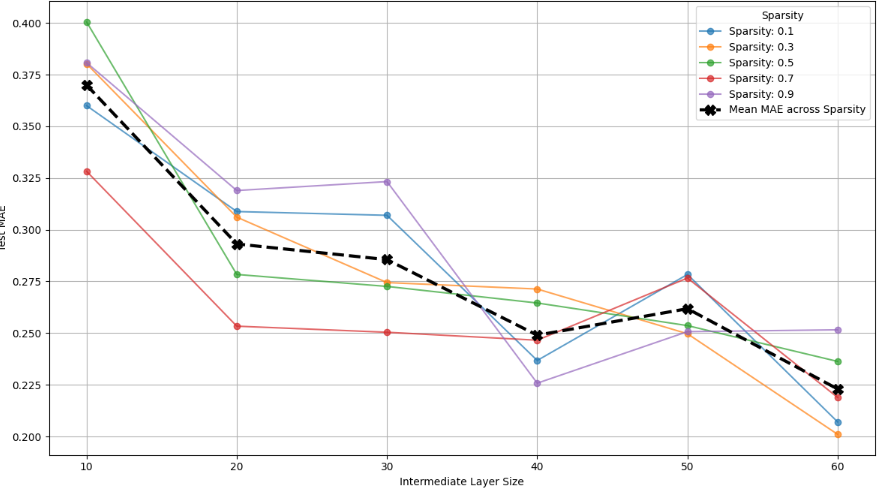
\includegraphics[height=7cm, width=13cm]{../img/sparcityhiddenlayer.png}
            \caption{Test MAE as a function of Intermediate Hidden Layer Size for different Sparsity values}
        \label{sparityhiddenlayer}                         
        \end{center}
\end{figure}


\begin{table}[htbp]
\centering
\caption{Error Distribution Comparison Between Standard ESN and MultiHead ESN}
\label{tab:esn_error_comparison}
\begin{tabular}{ccc}
\hline
\textbf{Error Range (cm)} & \textbf{ESN Count (\%)} & \textbf{MultiHead ESN Count (\%)} \\
\hline
$(-1, 1)$ & 39.80 & 76.65 \\
$(-2, 2)$ & 62.31 & 95.01 \\
$(-3, 3)$ & 76.72 & 98.38 \\
$(-4, 4)$ & 85.16 & 99.09 \\
\hline
\end{tabular}
\end{table}


The ESN estimator after training 1200 epochs produced a MAE of ~2cm with the percentage sample per error range shows in table \ref{tab:esn_error_comparison}, in order to further reduce the MAE of the ESN, it architecture was enhanced to use multihead feedforward network. The reason for this change comes from the observation that the ESN perform well as a clasifier, been capable to distinguish recording session near to each other, once the fedforward network was configured for the regresion task the errors in estimation were even larger that the distance betwen adyacent sessions, suggesting the possibility that the network was not able to learn the mapping function from the reservoir features to the output coordinates. A key diference between the clasification and regresion tasks is that the clasifier had an independent output for each class, but not only the output, it had an entire feedforward network in the form of a single layer perceptron for each class, so the network was able to learn a different mapping function for each class. The multihead feedforward network is a similar approach, but instead of having a single layer perceptron for each class, the learning task was dividen into three independent task, one network was dedicated to map the function for the positive coordinates, another for the negative coordinates and a third to predict the sign of the coordinate. The sign prediction network is resposable to select which of the other two networks will be used to predict the value of the coordinate. that provided a sustancial improvement in the performance of the ESN estimator. but still some small amount of estimation presented a large error in the case of misprediction of the sign of the coordinate, for this reason a forth network was proposed to estimate the value of the coordinate for the entire range of values, the output acuracy of this network is lower than the other arrangement, but is intended to be used as guidence for the other network, if the diference from estimation fromthe two networks is larger than a threshold, the network consider that a error inthe sign prediction network has ocurred andthe output is selected fromthe network of opposite sign. The architecture ofthe multihead feedforward network is shown in figure \ref{fig:multihead} and the results of the ESN estimator with this configuration is shown in table \ref{tab:esn_error_comparison} with a MAE of ~0.7cm and a significant improvement in the percentage of samples per error range.


\begin{figure}[htb]
        \begin{center}        
            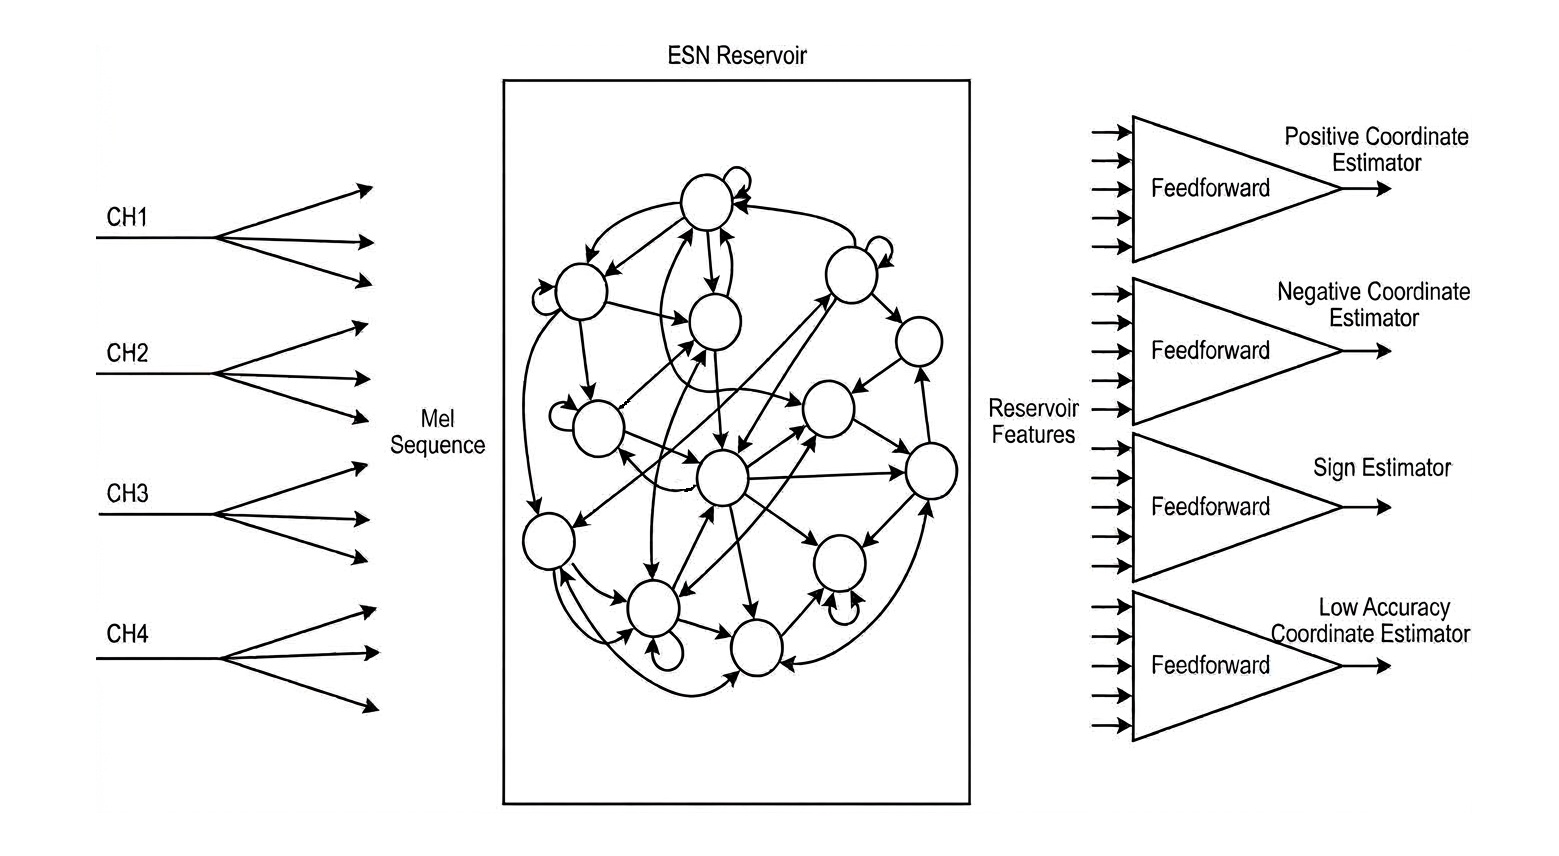
\includegraphics[height=8cm, width=15cm]{../img/Multi-Head_ESN_Estimator.jpg}
            \caption{Multihead Network architecture for the ESN Estimator.}
        \label{fig:multihead}                         
        \end{center}
\end{figure}

\subsection{ESN Training and Evaluation}

Each feedforward head was trained independently, the learning rate was set to $5e-5$ for all the sub-network heads, the batch size was set to 32. The training was perform separately for each head. The sub-heads for positive and negative coordinates were trained using only the samples with the corresponding sign, while the overall coordinate prediction head and the sign prediction head were trained using all the samples, the sub-heads for positive, negative and overall coordinate estimation were trained using Adam optimizationfor 400 epochs, while the sign prediction head was trained using Binary Cross entropy with Logits Loss for 800 epochs. The training process was performed using a five\-fold cross-validation approach, with four folds used for training and one fold reserved for testing, following an 80:20 percent ratio. The target values for X, Y and Z are normalized as described in section 5.1.3, and a denormalization step is applied to the output of the network to obtain the final coordinate estimations. The evaluation of the ESN consider the results of the four sub-heads using a hibrid aproach, the output selection rather than relying solely on a single prediction head, the final coordinate is computed through a decision tree. The sign head predicts the sign of the target Conditional Path Selection:If the predicted sign is positive, the positive head output is chosen.If negative, the negative head output is chosen. This yields a candidate coordinate estimation, referred to as the Conditional Path prediction.An outlier mitigation is also performed, if the absolute difference between the Overall Estimator prediction and the chosen Conditional Path prediction is calculated.If this difference exceeds a threshold (100 cm), indicating a potential critical sign classification failure, the model falls back to the alternate sign's estimator output to prevent high localization errors. the Algorith for the hibrid desition logic is shown in Algorith \ref{alg:hybrid_decision_logic}.



\begin{algorithm}[htbp]
\caption{Hybrid Decision Logic for Coordinate Estimation with Outlier Mitigation}
\label{alg:hybrid_decision_logic}
\begin{algorithmic}[1]
\Require Feature vector $\mathbf{x}$, Sign Head $\hat{s}(\cdot)$, Positive Head $\hat{y}_{+}(\cdot)$, Negative Head $\hat{y}_{-}(\cdot)$, Overall Estimator $\hat{y}_{\text{overall}}(\cdot)$, Outlier Threshold $\tau = 100\text{ cm}$
\Ensure Final Coordinate Estimation $\hat{y}$

\Statex \textbf{// Phase 1: Sign Classification}
\State $\text{pred\_sign} \gets \hat{s}(\mathbf{x})$ \Comment{Predicts whether target is positive or negative}

\Statex \textbf{// Phase 2: Conditional Path Selection}
\If{$\text{pred\_sign} \ge 0$} \Comment{Positive condition branch}
    \State $\hat{y}_{\text{cand}} \gets \hat{y}_{+}(\mathbf{x})$ \Comment{Candidate conditional path prediction}
    \State $\hat{y}_{\text{alt}} \gets \hat{y}_{-}(\mathbf{x})$  \Comment{Alternate path for fallback}
\Else \Comment{Negative condition branch}
    \State $\hat{y}_{\text{cand}} \gets \hat{y}_{-}(\mathbf{x})$
    \State $\hat{y}_{\text{alt}} \gets \hat{y}_{+}(\mathbf{x})$
\EndIf

\Statex \textbf{// Phase 3: Outlier Mitigation and Fallback Logic}
\State $\hat{y}_{\text{ref}} \gets \hat{y}_{\text{overall}}(\mathbf{x})$ \Comment{Evaluate baseline overall estimator}
\State $\Delta \gets |\hat{y}_{\text{ref}} - \hat{y}_{\text{cand}}|$ \Comment{Compute absolute discrepancy}

\If{$\Delta > \tau$} \Comment{Potential critical sign classification failure detected}
    \State $\hat{y} \gets \hat{y}_{\text{alt}}$ \Comment{Fallback to alternate estimator output}
\Else
    \State $\hat{y} \gets \hat{y}_{\text{cand}}$ \Comment{Retain candidate conditional path prediction}
\EndIf

\State \Return $\hat{y}$
\end{algorithmic}
\end{algorithm}


\section{Beamforming Implementation}

\section{Beamforming}

%Motivation for Beamforming

\subsection{Frequency Selection}

In order to implement beamforming using the audio channels, the principal spectral components of the source signal used as the stimulus within the measurement box must be analyzed. For this purpose, the Python "XXX" libraries are used, and the frequency response of the audio signal is plotted. The frequency response plot is shown in Figure \ref{fig:resfreqaudio}, while the top 10 frequencies with the highest magnitude are presented in Table \ref{tab:mainfreq}, where it can be observed that frequencies near 400\,Hz exhibit the largest magnitudes. Based on this, 400\,Hz is selected as the beamforming frequency.

\begin{figure}[!htb]
    \begin{center}
        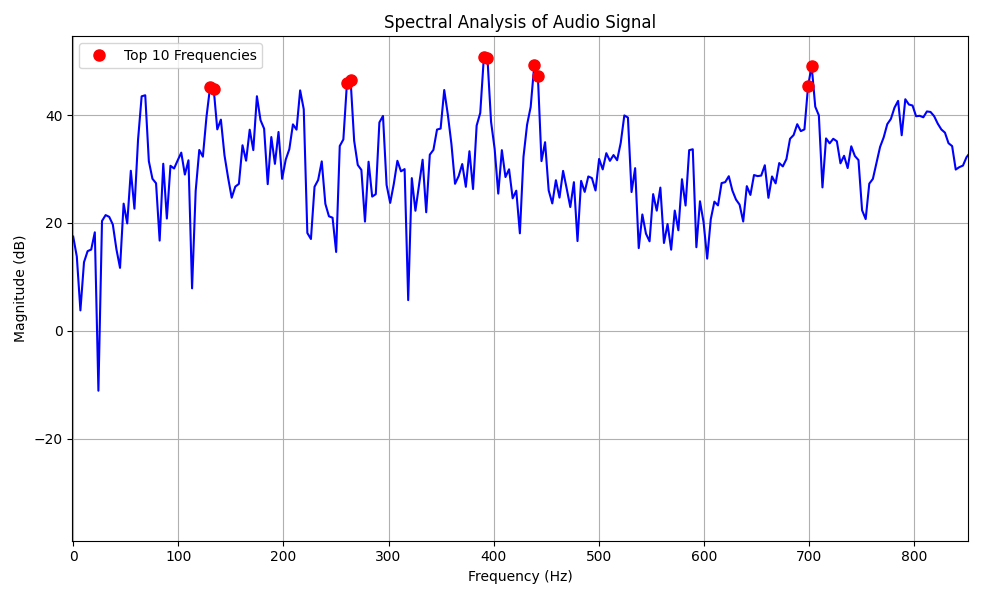
\includegraphics[height=9cm, width=13cm]{../img/mainfreq.png}
        \caption{Frequency response of the stimulus signal showing the top 10 spectral components with the highest magnitude.}
        \label{fig:resfreqaudio}
    \end{center}
\end{figure}

\begin{table}[h!]
\centering
\begin{tabular}{ccc}
\hline
\textbf{Rank} & \textbf{Frequency (Hz)} & \textbf{Magnitude (dB)} \\
\hline
1  & 390.72 & 50.71 \\
2  & 394.14 & 50.58 \\
3  & 438.70 & 49.31 \\
4  & 702.61 & 49.17 \\
5  & 442.13 & 47.26 \\
6  & 263.91 & 46.60 \\
7  & 260.48 & 45.96 \\
8  & 699.18 & 45.32 \\
9  & 130.24 & 45.19 \\
10 & 133.67 & 44.88 \\
\hline
\end{tabular}
\caption{Top 10 frequencies with the highest magnitude (dB).}
\label{tab:mainfreq}
\end{table}

Given that the microphones are placed in a plane parallel to the X-Z plane, forming pairs that enable binaural audition, measurements along the X and Z axes can serve as candidate inputs to evaluate the impact of beamforming on estimating the cube's position. A geometric analysis of the measurement box is required. In Figure \ref{fig:geometrybbox}, the midpoint of the sides perpendicular to the X-axis is defined as a location of interest. These points will be considered the acoustic source for the beamforming procedure. Assuming the sound originates from this point or surrounding regions, it is necessary to compute the path-length difference traveled by the same acoustic wave arriving at both microphones. Using trigonometry, the distance from point E to G is determined to be 0.522\,m, and the distance from E to H is 0.9862\,m. Their difference yields 0.4649\,m, which represents the extra distance the acoustic wave must travel to reach point H compared to point G. Assuming the speed of sound is 346\,m/s—the approximate speed at a temperature of 26\,$^{\circ}$C \cite{audiospeed}, which closely matches the average temperature at the testing site—the time difference of arrival (TDOA) between both microphones is 1.34\,ms, as expressed in Equation \ref{eq:Fa0}.

\begin{figure}[!htb]
    \begin{center}
        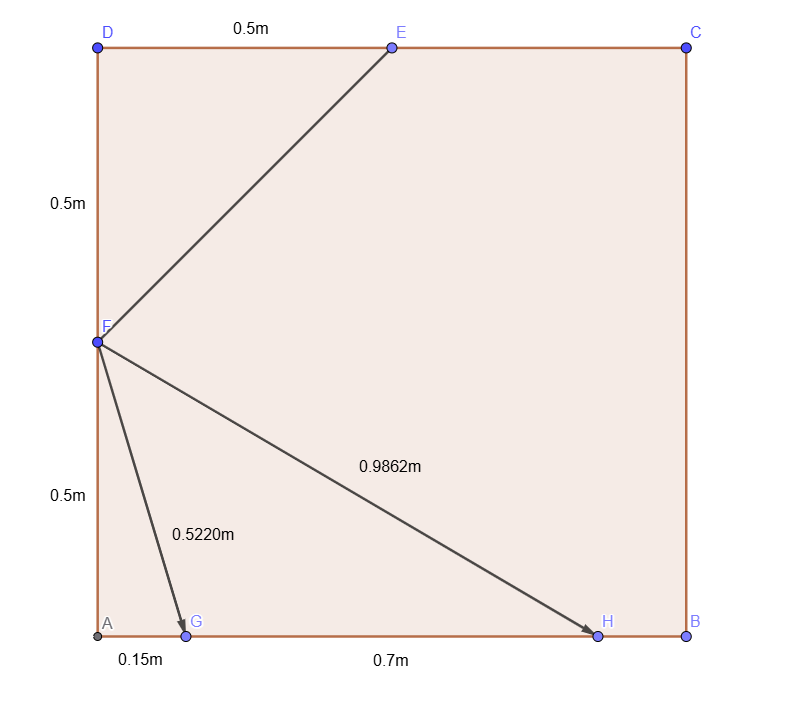
\includegraphics[height=12cm, width=13cm]{../img/Analisis_geometrico_BFM.png}
        \caption{Geometric layout of the measurement box illustrating the acoustic path from the speaker located at E to the microphones positioned at G and H.}
        \label{fig:geometrybbox}
    \end{center}
\end{figure}

\begin{equation} \label{eq:Fa0}
 \Delta t_{\text{arrival}} = \frac{0.4642\,\text{m}}{346\,\text{m/s}} = 1.34\,\text{ms}
\end{equation}

Selecting the highest-magnitude components around 400\,Hz for beamforming, combined with the computed time difference of arrival, enables an analysis of how the signal's main spectral components behave over the travel time $\Delta t$. At 400\,Hz, the signal period is 2.5\,ms. For a propagation delay $\Delta t = 1.35\,\text{ms}$ (as illustrated in Figure \ref{fig:ondas400}), the acoustic wave arrives at point G in an inverted-phase condition relative to point H, causing destructive cancellation when the two signals are summed. Consequently, introducing a delay equal to half the period (1.25\,ms) produces constructive interference for signals originating from point E at 400\,Hz. Furthermore, as the reverberant source shifts away from this target location, destructive attenuation penalizes the gain at these frequencies, fulfilling the objective of the beamforming operation.

\begin{figure}[!htb]
    \begin{center}
        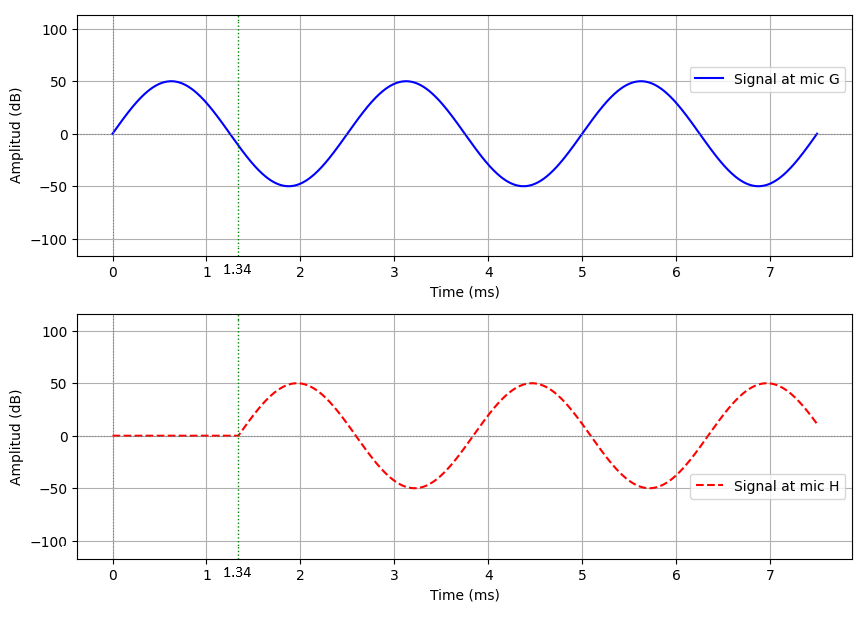
\includegraphics[height=9cm, width=13cm]{../img/signalbothmics.png}
        \caption{Acoustic waveforms at 400\,Hz captured by the microphones located at points G and H.}
        \label{fig:ondas400}
    \end{center}
\end{figure}


\subsection{Audio compactation}

\subsection{Limitations and Requirements}
A brief description of the design mechanism's limitations and requirements in accordance with the definitions in Scope and Limitations.